\subsubsection{Deciphering Transliterations - Background}

Transliteration is a mapping of terms between writing systems of different
languages. Usually, the transliterator tries to preserve the sounds
of the terms as they are spoken in the original language. For example,
the computer in Japanese as (``ko n pyu u ta a'' in romaji). The
``back-transliteration'' tasks is concerned with reversing the process
by restoring transliterated foreign words to their original script.

Knight and Graehl \cite{KG98} model the transliteration of English
terms $w$ to Japanese words $k$ by encoding a generative story as
a cascade of four finite state transducers (FST): 
\begin{enumerate}
\item First, a word $w$ is generated according to an English language model
$P[w]$
\item $w$ is then mapped to $(e_{1},\ldots,e_{M})$, a sequence of English
phonemes, according to a pronunciation model
\item Each phoneme $e_{m}$ is mapped to a sequence of Japanese phonemes
$j_{m}$ according to phoneme mapping model $P[j_{m}\mid e_{m}]$
(limited to 1-to-1 and or 1-to-2 phoneme mappings)
\item Finally, the entire Japanese pronunciation sequence is mapped to a
Japanese word $k$ in Katakana script
\end{enumerate}
\cite{KG98} construct and train these FSTs independently. In particular,
to train the phoneme mapping model $P[j_{m}\mid e_{m}]$ a parallel
phoneme corpus is provided $\{(w_{n},\, k_{n})\}$ and the likelihood
of the observed data is maximized using EM.

Ravi and Knight \cite{RK09} extend this formulation to the significantly
more difficult setting of decipherment, where no parallel data is
provided. In this case, only the Japanese words $\{k_{n}\}$ are observed,
without their English counterparts. An observed Japanese word $k$
can then be explained by all possible English words $w$ that could
have generated it, via the equation $P[k]=\sum_{w}P[w]\cdot P[k\mid w]$.
In training, the $P[j_{m}\mid e_{m}]$ parameters are estimated, while
the other FSTs remain fixed.

\cite{RK09} compare back-transliteration whole name error rates on
a list of 100 US senator names. They report a 40\% error rate in the
parallel setting, and a 73\% error rate when using their best decipherment
setting. Inspecting the learned phoneme mapping model $P[j_{m}\mid e_{m}]$
in both cases, it is clear that EM in the parallel data settings learns
sparse and peaked distributions per each phoneme. Overall, less than
200 parameters have value larger than 0.01 in the parallel case, while
in decipherment, the number orders on 400. As expected, ordinary EM
leaves a lot of room for ambiguity in the decipherment case.

% Preview source code for paragraph 31

\begin{tabular}{ccc}
 &  & \tabularnewline
 & 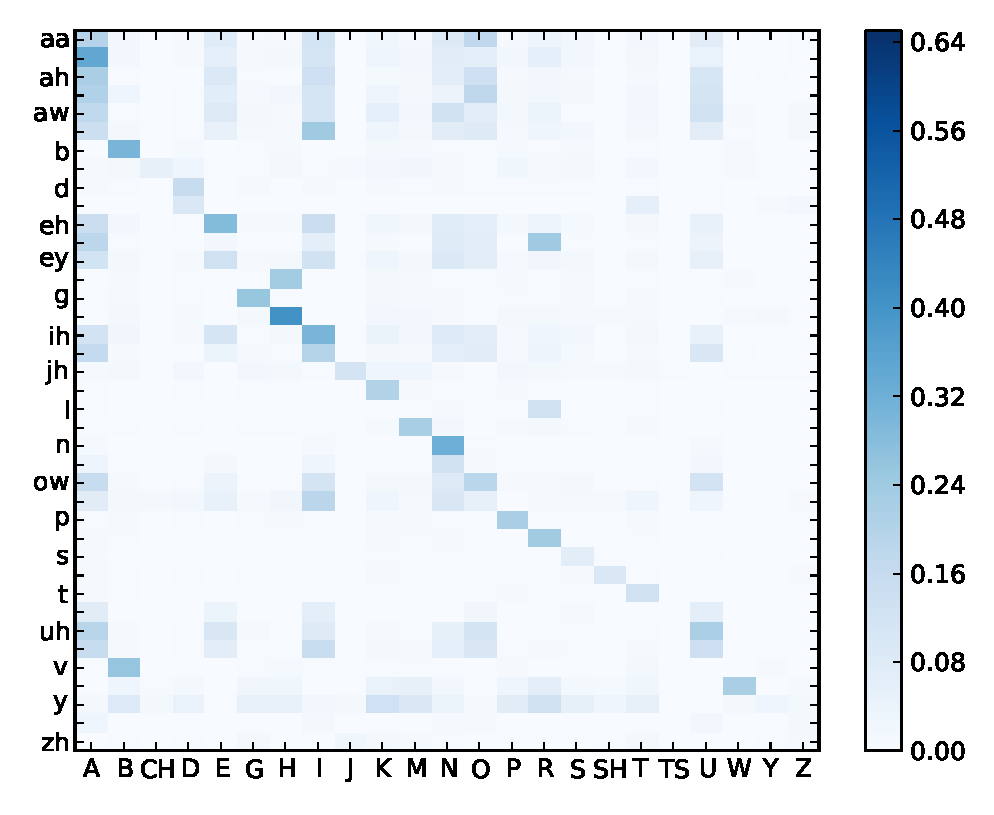
\includegraphics[scale=0.4]{figures/model_11_vanilla} & \includegraphics[scale=0.4]{figures/model_11_gm}\tabularnewline
 &  & \tabularnewline
\end{tabular}


\subsubsection{Deciphering Transliterations - Experiments}

To 
\begin{itemize}
\item no Parallel Data
\item Fair Experiment setting

\begin{itemize}
\item Data Collection, Numbers
\item Generate the entire LM both ways.
\item Comparison of results and sparsity, image for sparsity
\end{itemize}
\end{itemize}